%%%%%%%%%%%%%%%%%%%%%%%%%%%%%%%%%%%%%%%%%
% Short Sectioned Assignment
% LaTeX Template
% Version 1.0 (5/5/12)
%
% This template has been downloaded from:
% http://www.LaTeXTemplates.com
%
% Original author:
% Frits Wenneker (http://www.howtotex.com)
%
% License:
% CC BY-NC-SA 3.0 (http://creativecommons.org/licenses/by-nc-sa/3.0/)
%
%%%%%%%%%%%%%%%%%%%%%%%%%%%%%%%%%%%%%%%%%

%----------------------------------------------------------------------------------------
%	PACKAGES AND OTHER DOCUMENT CONFIGURATIONS
%----------------------------------------------------------------------------------------

\documentclass[paper=a4, fontsize=11pt]{scrartcl} % A4 paper and 11pt font size

\usepackage[T1]{fontenc} % Use 8-bit encoding that has 256 glyphs
\usepackage{fourier} % Use the Adobe Utopia font for the document - comment this line to return to the LaTeX default
\usepackage[english]{babel} % English language/hyphenation
\usepackage{amsmath,amsfonts,amsthm} % Math packages

\usepackage{lipsum} % Used for inserting dummy 'Lorem ipsum' text into the template
\usepackage{bbding}
\usepackage{multirow}
\usepackage{caption}
\usepackage{graphicx}
\usepackage{hyperref}

\usepackage{sectsty} % Allows customizing section commands
\allsectionsfont{\centering \normalfont\scshape} % Make all sections centered, the default font and small caps

\usepackage{fancyhdr} % Custom headers and footers
\pagestyle{fancyplain} % Makes all pages in the document conform to the custom headers and footers
\fancyhead{} % No page header - if you want one, create it in the same way as the footers below
\fancyfoot[L]{} % Empty left footer
\fancyfoot[C]{} % Empty center footer
\fancyfoot[R]{\thepage} % Page numbering for right footer
\renewcommand{\headrulewidth}{0pt} % Remove header underlines
\renewcommand{\footrulewidth}{0pt} % Remove footer underlines
\setlength{\headheight}{13.6pt} % Customize the height of the header

\numberwithin{equation}{section} % Number equations within sections (i.e. 1.1, 1.2, 2.1, 2.2 instead of 1, 2, 3, 4)
\numberwithin{figure}{section} % Number figures within sections (i.e. 1.1, 1.2, 2.1, 2.2 instead of 1, 2, 3, 4)
\numberwithin{table}{section} % Number tables within sections (i.e. 1.1, 1.2, 2.1, 2.2 instead of 1, 2, 3, 4)

\setlength\parindent{0pt} % Removes all indentation from paragraphs - comment this line for an assignment with lots of text

\usepackage{amsmath}

%----------------------------------------------------------------------------------------
%	TITLE SECTION
%----------------------------------------------------------------------------------------

\newcommand{\horrule}[1]{\rule{\linewidth}{#1}} % Create horizontal rule command with 1 argument of height

\title{	
\normalfont \normalsize 
\textsc{} \\ [25pt] % Your university, school and/or department name(s)
\horrule{0.5pt} \\[0.4cm] % Thin top horizontal rule
\huge Evaluation of Early Stopping in A/B Testing  \\ % The assignment title
\horrule{2pt} \\[0.5cm] % Thick bottom horizontal rule
}

\author{Shan Huang} % Your name

\date{\normalsize\today} % Today's date or a custom date

\begin{document}

\maketitle % Print the title

%----------------------------------------------------------------------------------------
%	PROBLEM 1
%----------------------------------------------------------------------------------------

This documentation shows the evaluation of early stopping algorithms. 

\section{Problem}
Given samples $\textbf{x}$ from treatment group, samples $\textbf{y}$ from control group, we want to know whether there is a significant difference between the means $\delta = \mu(y)-\mu(x)$.

To save the cost of long-running experiments, we want to stop the test early if we are already certain that there is a statistically significant result.

\section{Significance Decision}
\label{sec:byt}
We can decide whether the difference is statistically significant using either:

\begin{itemize}  
\item \textbf{Confidence interval}: If 0 is outside confidence interval of $\delta$, it is statistically significant.
\item or \textbf{credible interval}: Credible interval is the Bayesian version of confidence interval. If 0 is outside credible interval of $\delta$, it is statistically significant.
\item or \textbf{Bayes factor}: Theoretically, Bayes factors higher than 3 can be interpreted as support for the null hypothesis (significant no difference), whereas values smaller than 1/3 can be interpreted as support for the alternative hypothesis (significant difference). Values between 1/3 and 3 are inconclusive. \textbf{In our test, we will only use Bayes factor less than 1/3 as decision criteria}. See reasons below.
\end{itemize}

Given the null hypothesis $H_0$ representing no difference, the alternative hypothesis $H_1$ representing a difference of the means, the ability of each metric, i.e., types of significance it can detect, is shown in the following table.
\begin{center}
  \begin{tabular}{ | r | c | c | c | c | }
    \hline
    & Paradigm & Significant $H_1$ & Significant $H_0$ & No Significant Result \\ \hline
    \textbf{Confidence Interval} & frequentist &  \Checkmark &  & \Checkmark\\ \hline
    \textbf{Credible Interval} & Bayesian & \Checkmark &  & \Checkmark\\ \hline
    \textbf{Bayes factor} & Bayesian & \Checkmark & \Checkmark & \Checkmark\\
    \hline
  \end{tabular}
\captionof{table}{Comparison of Decision Ability}
\end{center}

To be consistent with all mehods, we draw a binary conclusion that either there is a significant difference or not. In other words, the first column means that there is a significant difference, combining the second and third column means that there is no significant difference. Thus, we only use the part where Bayes factor less than 1/3 as decision criteria.

It is worth noting that a \textbf{typical conclusion of Bayes factor} would be "\emph{There is a significant difference corresponds to Cauchy prior and a threshold of Bayes factor=3}". This might be quite difficult to explain to non-tech users. While the \textbf{conclusion based on interval} can be more intuitive such as "\emph{You can be 95\% sure that the significant difference is not due to chance}".


\section{Early Stopping Criteria}
We can stop the experiment by either
\begin{itemize}  
\item \textbf{Confidence interval}: Calculate the new significance level for each day based on alpha-spending function in group sequential method. Stop the test If 0 is outside confidence interval of $\delta$. 
\item or \textbf{credible interval}: Stop the test if 0 is outside credible interval of $\delta$.
\item or \textbf{Bayes factor}: Stop the test if Bayes factor is smaller than 1/3 (significant difference).
\item or \textbf{Bayes precision}: Stop the test if credible interval width is smaller than 0.08. 
\end{itemize}


\section{Metric}

\subsection{Evaluate Significance Decision}
We are going to compare false positive(type I error), false negative(type II error), true positive, true negative rates for the three significance decision criteria described in Section ~\ref{sec:byt}.

\subsection{Evaluate Early Stopping Criteria}
\label{sec:esc}
It is obvious that if we use the frequentist approach in early stopping, we should also use frequentist's approach (that is confidence interval) to decide significance. Moreover, when using Bayes factor to stop, we often find a conflicting result if we draw significance conclusion based on credible interval. Therefore we don't evaluate all combinations of early stopping algorithms and significance decision algorithms, find below a table of combination we will evaluate.

\begin{center}
  \begin{tabular}{ | r | c | c | c | c | }
    \hline
    \multirow{2}{*}{Significant Based On} & \multicolumn{4}{ |c| }{Early Stopping Based On} \\ \cline{2-5}
    & Confidence Interval & Credible Interval & Bayes factor & Bayes precision \\ \hline
    Confidence Interval & \Checkmark & &  &  \\ \hline
    Credible Interval &  & \Checkmark &  &  \\ \hline
    Bayes factor &  & & \Checkmark & \Checkmark \\ \hline
  \end{tabular}
\captionof{table}{Combinations of Early Stopping and Significance Decision To Evaluate}
\end{center}

For each combination shown in the table above, we will evaluate the following metrics:
\begin{itemize}  
\item \textbf{False positive rate}: Percentage of tests which are wrongly stopped. i.e., Early stop says there is a significant difference and stops the test, but the test to the end day (as if there is no early stopping) will tell you it is not significant.
\item \textbf{Run time reduced(all)}: Percentage of run time reduced for all tests.
\item \textbf{Run time reduced(true positive)}: Percentage of run time reduced for only the correctly stopped tests.
\item \textbf{Bias}: Difference of effect size(delta) between stopping day and end day of test(as if there is no early stopping).
\end{itemize}

\section{Evaluation}

The evaluation is conducted on both simulation data and real data. Code can be found \href{https://github.com/shansfolder/ABTestingEarlyStoppingEvaluation}{\underline{here}}.

\subsection{Simulation Data}
We generate 2000 simulation tests based on Gaussian distributed KPIs. We calculate the minimal detectable effect size from power analysis. 1000 tests have a significant difference between control and treatment, and the other 1000 tests have no significant difference. 

We model the frequency of visits of an entity by a Poisson distribution with 3 days per entity in average. We simulate the A/B testing for a period of 20 days, and decide whether to stop on each day.

First of all, let's see the performance of different \textbf{significance decision} algorithms.
\begin{center}
  \begin{tabular}{ | r | c | c | c | c | }
    \hline
    & FPR & TNR & FNR & TPR \\ \hline
    \textbf{confidence interval} & 4.6\% & 95.4\% & 0.9\% & 99.1\% \\ \hline
    \textbf{credible interval} & 4.6\% & 95.4\% & 1.0\% & 99.0\% \\ \hline
    \textbf{Bayes factor} & 0.2\% & 99.8\% & 18.9\% & 81.1\%\\
    \hline
  \end{tabular}
\captionof{table}{Performance of Significance Decision on Simulation Data}
\end{center}

We can observe in Figure \ref{fig:roc_sim_data} that Bayes factor works very good on false positive rate, but the two interval based approaches works better on true positive rate. In general, the two interval based approaches are a little bit better because of larger distances to the line of random guess, while the error rate of all three methods are acceptable(FPR < 5\% and FNR < 80\%). 

\begin{figure} 
\centering
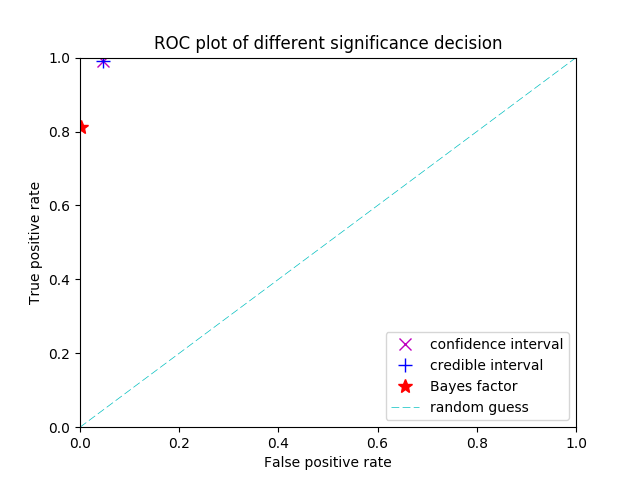
\includegraphics[scale=.6]{roc_sim_data.png}
\caption{ROC plot on simulation data}
\label{fig:roc_sim_data}
\end{figure}

Next, let's look at the results of \textbf{early stopping} algorithms. To make notations compact, in the following table we use FPR for false positive rate, RTR(all) for run time reduced(all), RTR(TP) for run time reduced(true positive) and CI for confidence interval. The definition of each metric is described previously in Section ~\ref{sec:esc}.

\begin{center}
  \begin{tabular}{ | r | r | c | c | c | c | c | }
    \hline
    \textbf{Significance} & \textbf{Early Stopping}  & \textbf{Paradigm} & \textbf{FPR} & \textbf{RTR(all)} & \textbf{RTR(TP)} & \textbf{Bias} \\ \hline\hline
    CI &  CI & frequentist & 3.3\% &  1.60\% & 16.74\% & 0.00 \\ \hline
    Credible Interval & Credible Interval & Bayesian & \textbf{22.6}\% & 17.56\% &  42.28\% & 0.00 \\ \hline
    Bayes factor & Bayes factor & Bayesian & 0.7\% & 0.57\% & 42.5\% & -0.02 \\ \hline
    Bayes factor & Bayes precision & Bayesian & 0.2\% & 78.02\% &  78.02\% &  0.00 \\ \hline
  \end{tabular}
\captionof{table}{Performance of Early Stopping in A/A test on Simulation Data}
\end{center}

\begin{center}
  \begin{tabular}{ | r | r | c | c | c | c | c | }
    \hline
    \textbf{Significance} & \textbf{Early Stopping}  & \textbf{Paradigm} & \textbf{FPR} & \textbf{RTR(all)} & \textbf{RTR(TP)} & \textbf{Bias} \\ \hline\hline
    CI &  CI & frequentist &1.7\% & 51.58\% & 51.74\% & -0.01 \\ \hline
    Credible Interval & Credible Interval & Bayesian & 0.7\% & 78.53\% & 78.78\% & 0.00 \\ \hline
    Bayes factor & Bayes factor & Bayesian & 7.8\% & 46.44\% & 52.96\% & 0.00 \\ \hline
    Bayes factor & Bayes precision & Bayesian & \textbf{67.8}\% & 77.95\% & 77.76\% & -0.02 \\ \hline
  \end{tabular}
\captionof{table}{Performance of Early Stopping in A/B test on Simulation Data}
\end{center}




\subsection{Real Data}
ToDo: Repeat the evaluation process on real data from previous A/B testings.

\section{Conclusion}
ToDo: Choose a significance decision criteria and an early stopping algorithm.
%Use group sequential and confidence interval.

%----------------------------------------------------------------------------------------

\end{document}